\documentclass[11pt]{article}
\usepackage[utf8]{inputenc}
\usepackage[T1]{fontenc}
\usepackage{amsmath}
\usepackage{booktabs}
\usepackage{graphicx}
\usepackage{geometry}
\usepackage{hyperref}
\geometry{margin=1in}
\graphicspath{{../outputs/figures/}}

\title{Portugal's General-Government Balance by Subsector, 1977--2025}
\author{Diogo Ribeiro}
\date{}

\begin{document}
\maketitle

\section*{Abstract}

This report decomposes Portugal's annual general-government net lending (+) / net borrowing (-) into Central Government, Regional and Local Government, and Social Security Funds (SSF). The analysis is empirical and accounting-focused. It studies long-run balance composition, year-to-year attribution, revenue and expenditure dynamics, persistence, structural mean shifts, Social Security revenue composition, primary balances, public investment, debt-flow reconciliation, and descriptive macroeconomic co-movement.

The central accounting identity is

\[
B^{GG}_t = B^{C}_t + B^{RL}_t + B^{SSF}_t.
\]

No causal, normative, or policy-intent interpretation is assigned to this identity.

\section{Data and Reproducibility}

The balance panel covers \textbf{1977--2025}, or \textbf{49 annual observations}. Historical data come from the Banco de Portugal / INE long series. The continuous modern balance bridge uses INE data distributed through PORDATA, while the CFP ESA 2010 workbooks provide modern revenue, expenditure, interest, investment, debt and stock-flow data.

The known statistical splice at \textbf{1995} is retained explicitly. No smoothing is applied across it. Detailed subsector revenue/expenditure accounts are available for 1977--1995 in the historical source and 2000--2025 in the modern CFP source; \textbf{1996--1999 are therefore left missing rather than imputed}.

\begin{center}
\resizebox{\linewidth}{!}{%
\begin{tabular}{@{}llll@{}}
\toprule
Sector & First year & Last year & Observations \\
\midrule
central\_government & 1977 & 2025 & 45 \\
general\_government & 1977 & 2025 & 49 \\
regional\_local\_government & 1977 & 2025 & 45 \\
social\_security\_funds & 1977 & 2025 & 45 \\
\bottomrule
\end{tabular}%
}
\end{center}

The maximum absolute subsector closure error in the canonical balance panel is \textbf{1.00 M EUR}. The maximum revenue-minus-expenditure account identity error is \textbf{0.000000 M EUR}. The modern debt-flow reconciliation closes with a maximum absolute error of \textbf{0.000000 M EUR}.

\section{Long-Run Subsector Decomposition}

\begin{figure}[htbp]
\centering
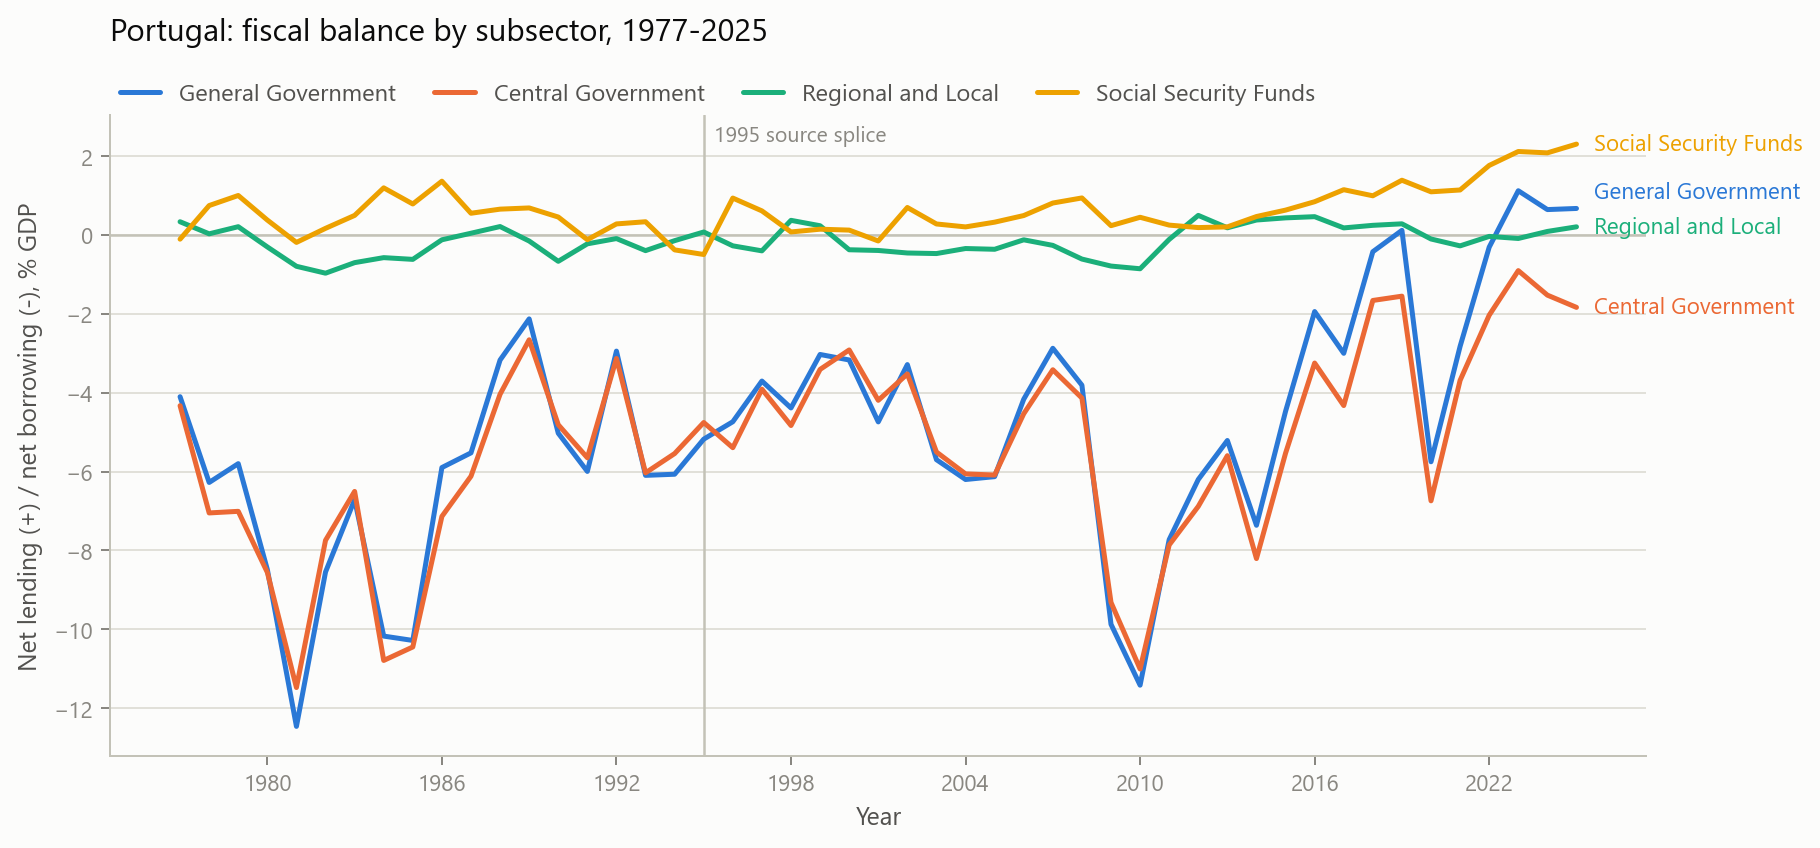
\includegraphics[width=\linewidth]{01_long_run_balances.png}
\caption{Long-run balances by subsector.}
\end{figure}

Across the full 1977--2025 balance panel, the aggregate General Government balance is positive in \textbf{4 years: 2019, 2023, 2024, 2025}. The table below reports sign persistence and balance magnitudes by subsector.

\begin{center}
\resizebox{\linewidth}{!}{%
\begin{tabular}{@{}llllllll@{}}
\toprule
Sector & N & Positive years & Negative years & Mean (\% GDP) & Median (\% GDP) & Longest positive run & Longest negative run \\
\midrule
general\_government & 49 & 4 & 45 & -4.915 & -5.028 & 3 & 42 \\
central\_government & 49 & 0 & 49 & -5.381 & -5.396 & 0 & 49 \\
regional\_local\_government & 49 & 18 & 31 & -0.157 & -0.124 & 8 & 12 \\
social\_security\_funds & 49 & 43 & 6 & 0.623 & 0.495 & 24 & 2 \\
\bottomrule
\end{tabular}%
}
\end{center}

The Central Government balance is negative in \textbf{49 of 49 observations} in the canonical balance series. By contrast, SSF has a positive balance in \textbf{43 observations}. These are descriptive frequencies, not counterfactual statements about what the aggregate balance would have been under a different institutional arrangement.

\subsection{Positive Aggregate-Balance Years}

\begin{center}
\resizebox{\linewidth}{!}{%
\begin{tabular}{@{}lllllll@{}}
\toprule
Year & GG balance (M EUR) & Central (M EUR) & Regional/local (M EUR) & SSF (M EUR) & Non-SSF (M EUR) & SSF offset ratio \\
\midrule
2019 & 249.000 & -3,331.000 & 604.000 & 2,975.000 & -2,727.000 & 1.091 \\
2023 & 3,030.000 & -2,447.000 & -243.000 & 5,720.000 & -2,690.000 & 2.126 \\
2024 & 1,863.000 & -4,424.000 & 256.000 & 6,031.000 & -4,168.000 & 1.447 \\
2025 & 2,059.000 & -5,636.000 & 630.000 & 7,065.000 & -5,006.000 & 1.411 \\
\bottomrule
\end{tabular}%
}
\end{center}

In 2025, the identity is

\[
2059
=
-5636
+
630
+
7065
\quad \text{M EUR}.
\]

The combined non-SSF balance is \textbf{-5006 M EUR}, while the SSF offset ratio is \textbf{1.411}. The ratio is defined as SSF balance divided by the absolute value of the negative non-SSF balance whenever those signs make the ratio meaningful.

\begin{figure}[htbp]
\centering
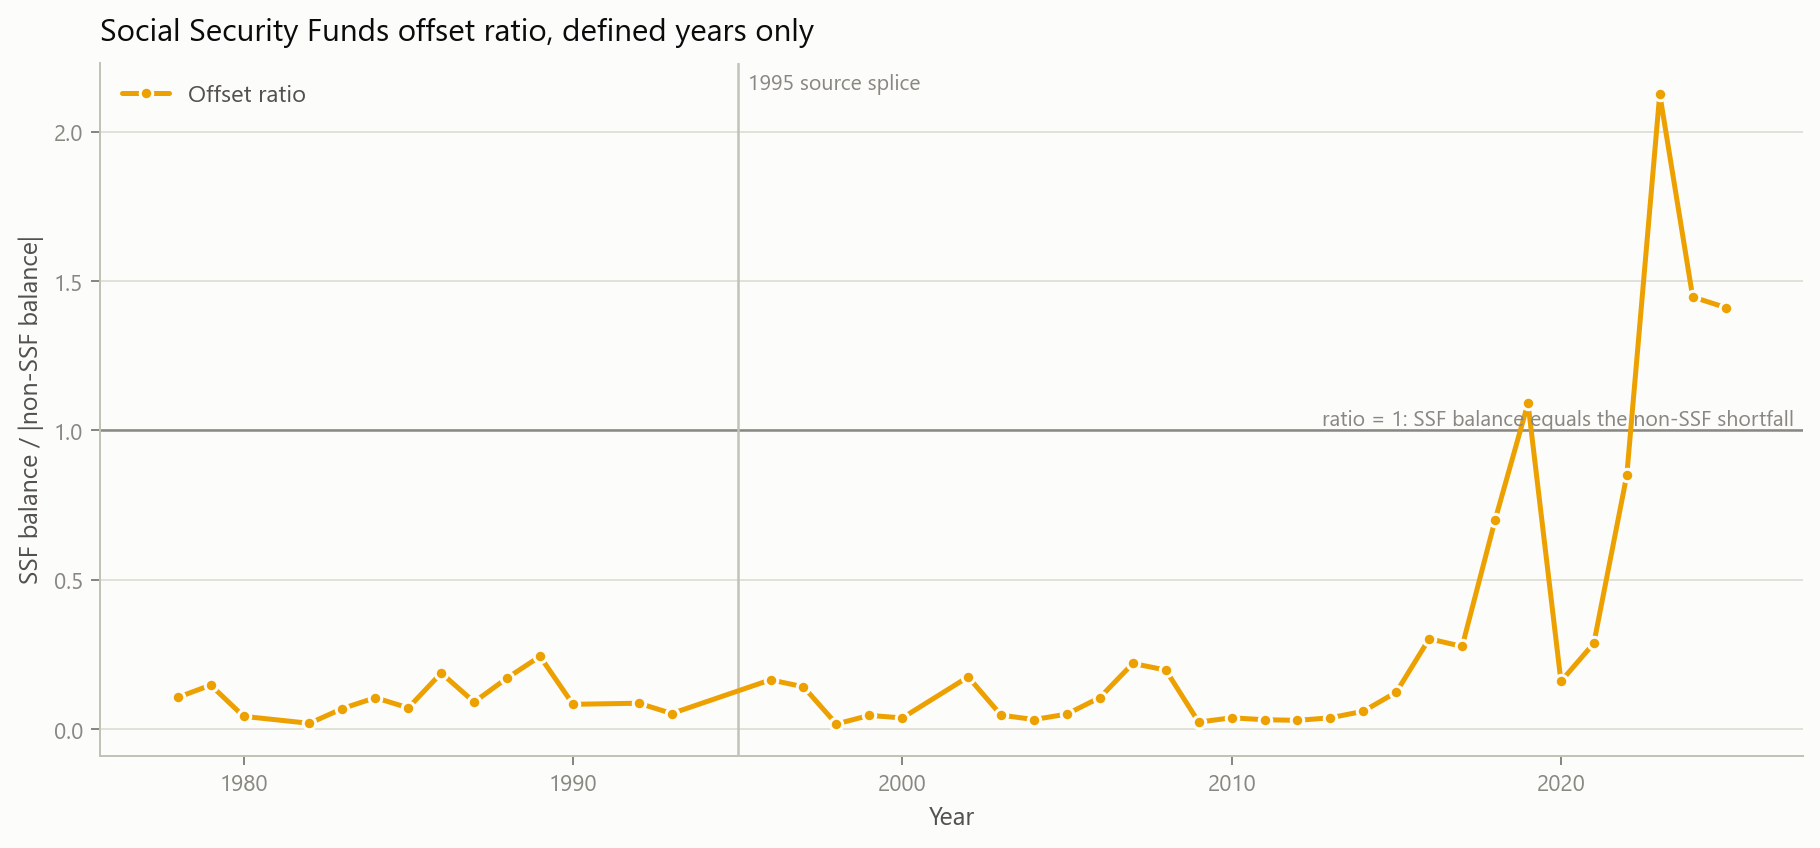
\includegraphics[width=\linewidth]{02_ssf_offset_ratio.png}
\caption{Social Security Funds offset ratio.}
\end{figure}

\section{Year-to-Year Attribution}

The annual change in the aggregate balance can be written exactly as

\[
\Delta B^{GG}_t
=
\Delta B^{C}_t
+
\Delta B^{RL}_t
+
\Delta B^{SSF}_t.
\]

The repository stores this decomposition for every adjacent year in \path{outputs/tables/balance_change_attribution.csv}. This distinguishes the level of a subsector balance from its contribution to an annual improvement or deterioration.

\begin{figure}[htbp]
\centering
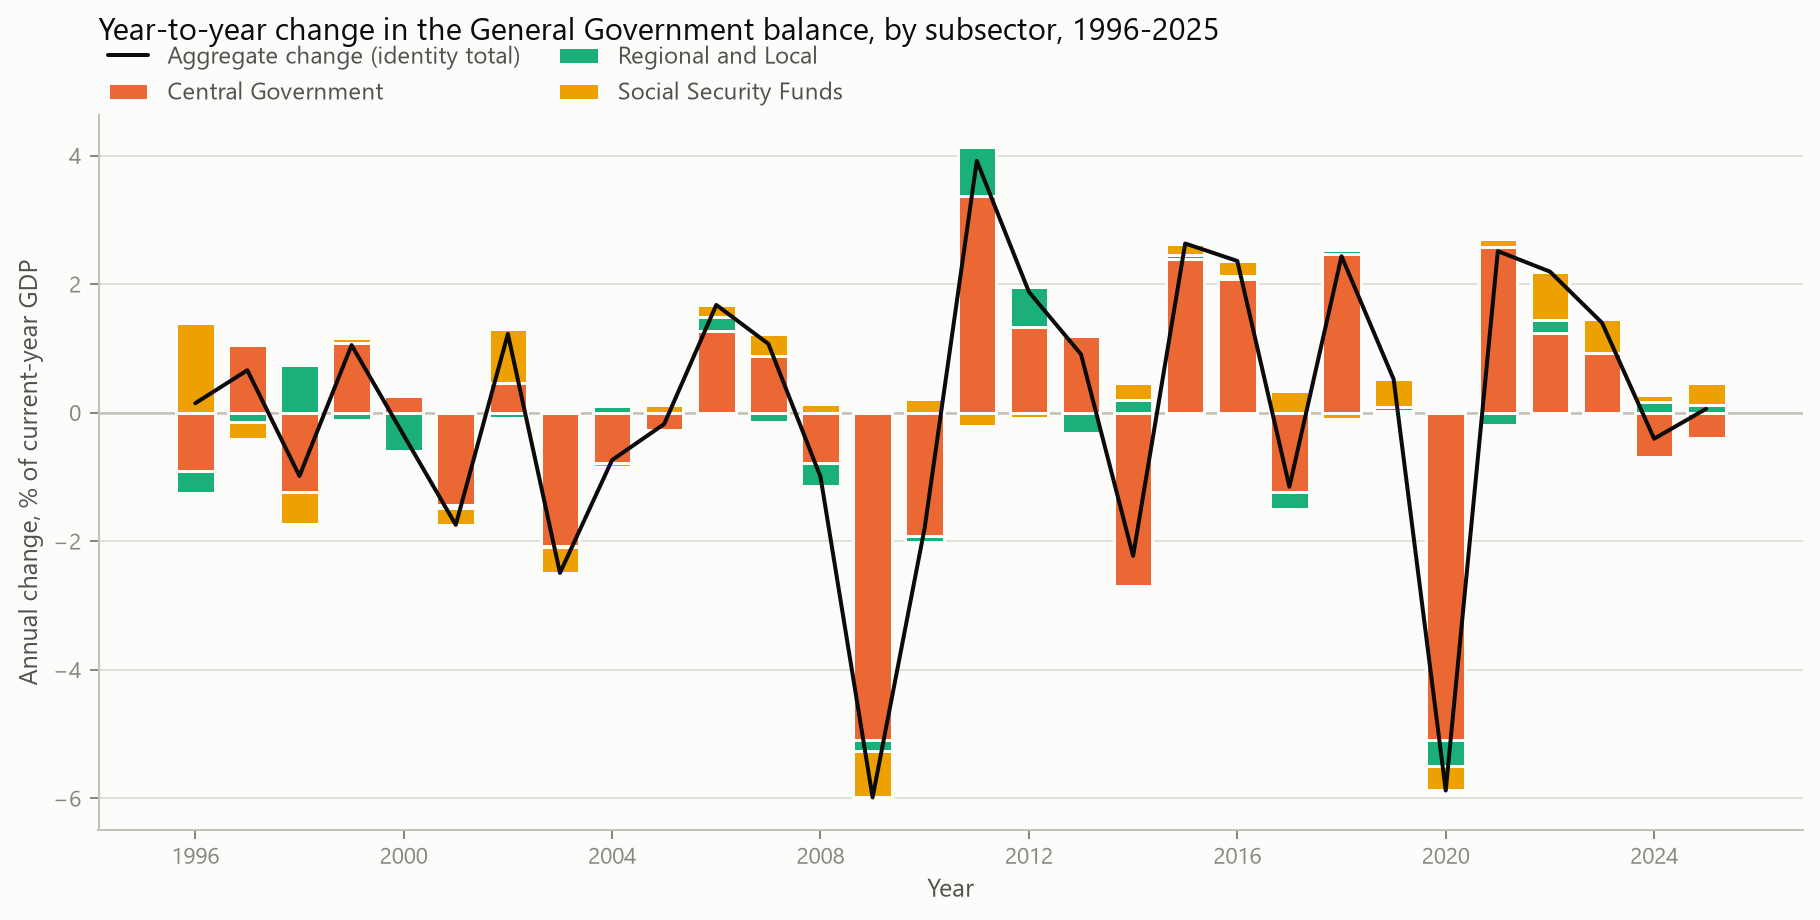
\includegraphics[width=\linewidth]{03_balance_change_attribution.png}
\caption{Annual balance-change attribution.}
\end{figure}

\section{Revenue and Expenditure Dynamics}

For every sector-year with detailed accounts, the balance is decomposed as

\[
B_{i,t} = R_{i,t} - E_{i,t},
\]

and therefore

\[
\Delta B_{i,t} = \Delta R_{i,t} - \Delta E_{i,t}.
\]

The exact annual decomposition is stored in \path{outputs/tables/revenue_expenditure_change_decomposition.csv}. Source gaps are not bridged when calculating changes.

\begin{figure}[htbp]
\centering
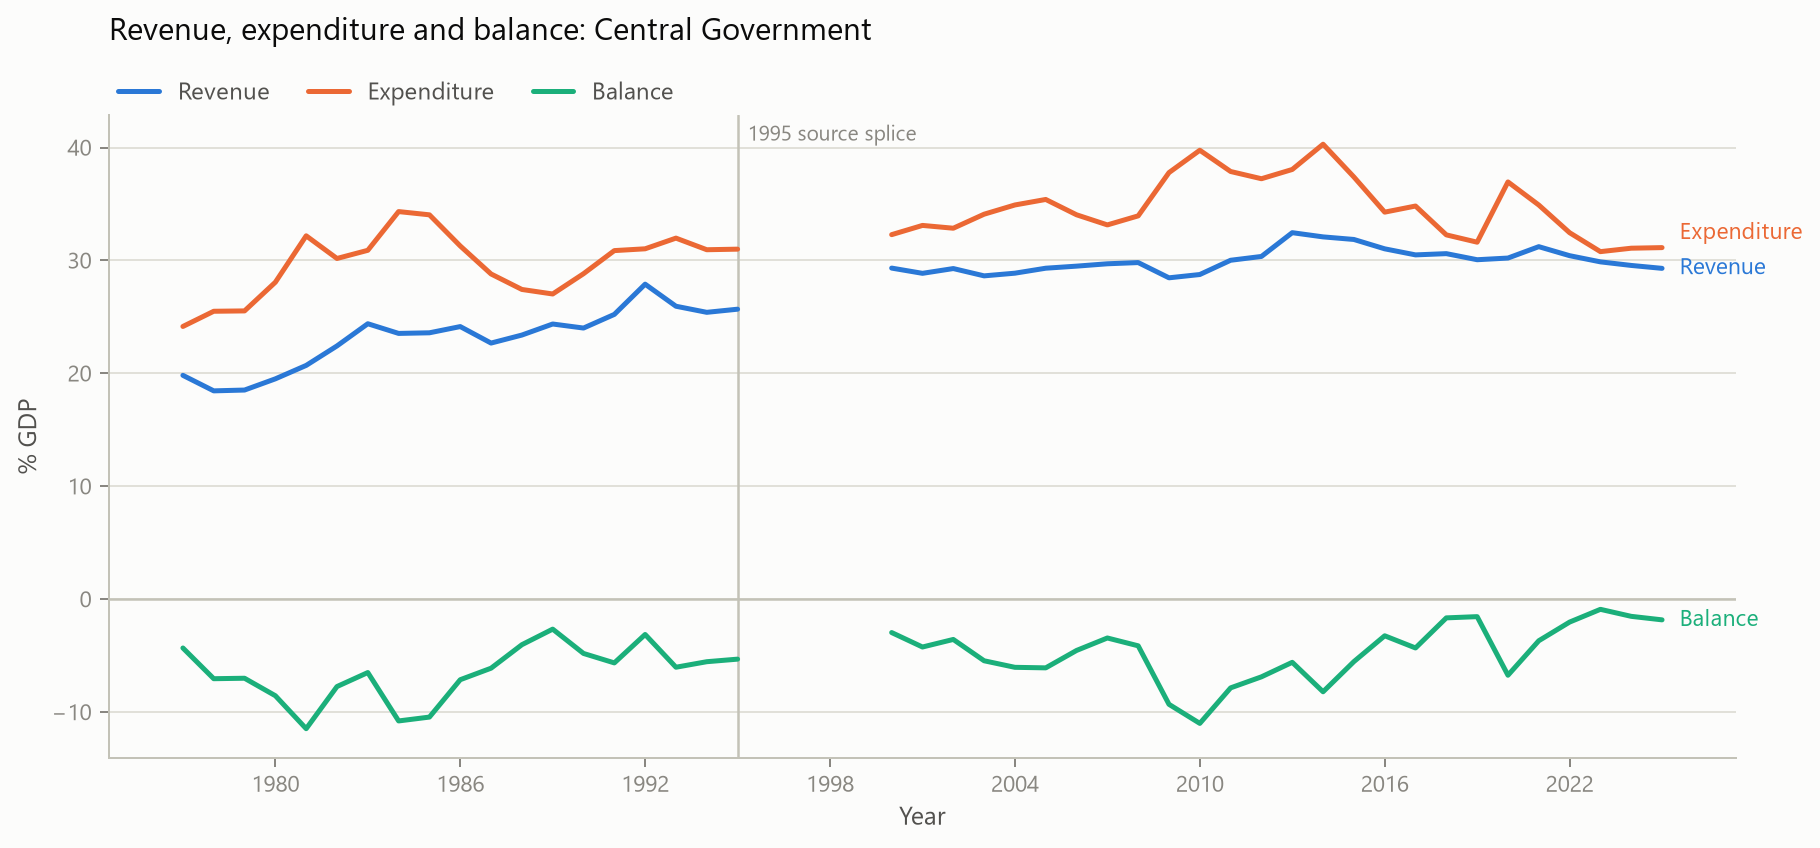
\includegraphics[width=\linewidth]{04_central_revenue_expenditure.png}
\caption{Central Government revenue and expenditure.}
\end{figure}

\section{Social Security Funds: Revenue Composition and Internal Systems}

The long-run SSF account series contains total revenue, total expenditure and social contributions. In 2025, social contributions were \textbf{67.07\% of total SSF revenue} in the ESA 2010 account table.

\begin{figure}[htbp]
\centering
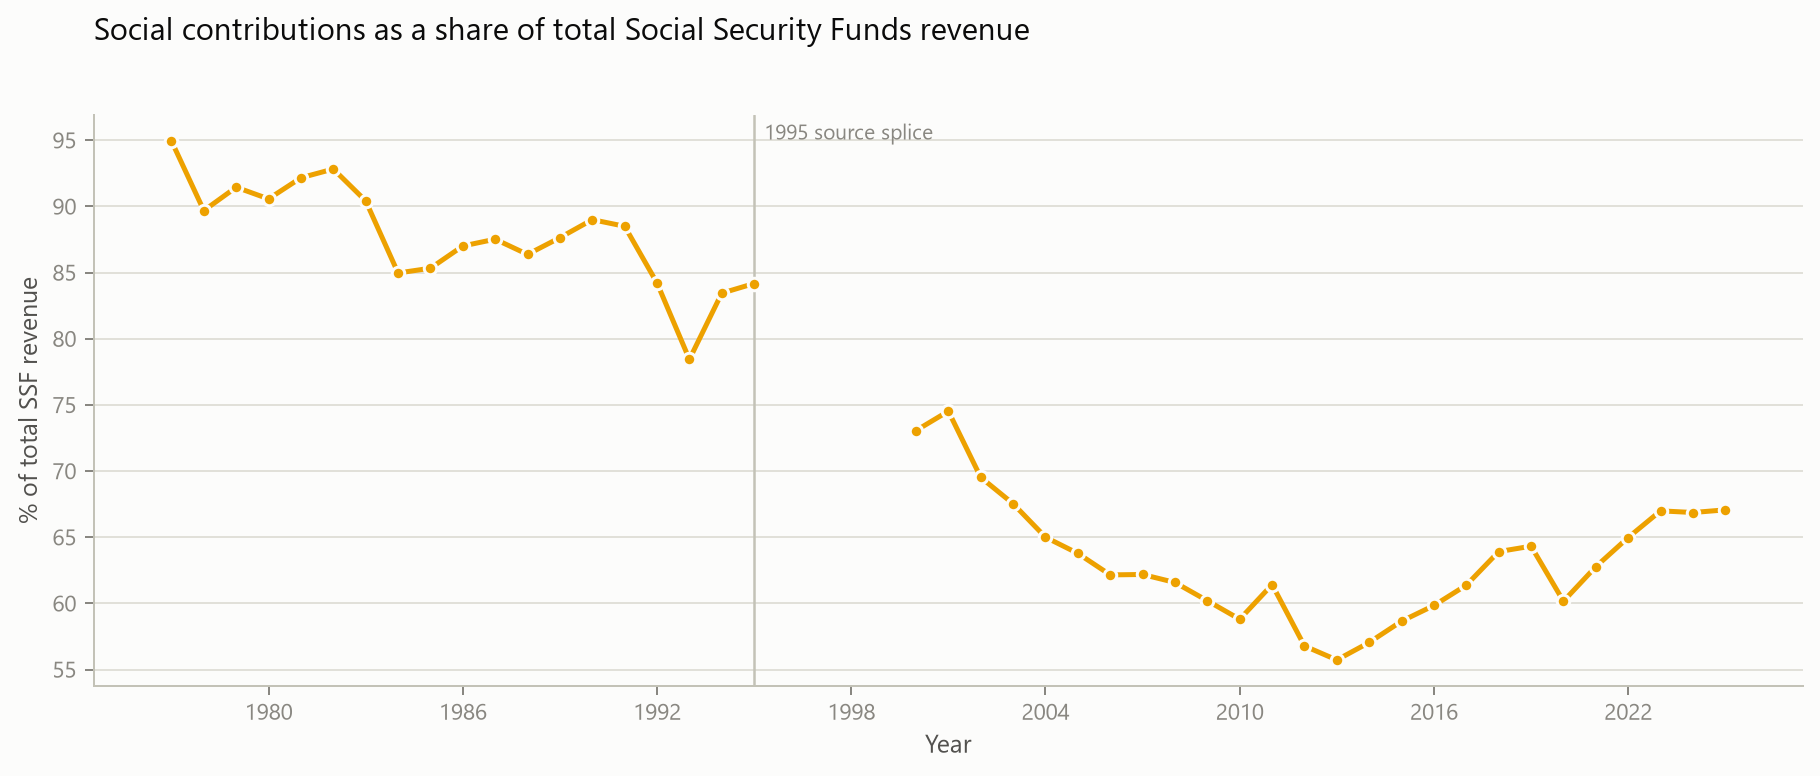
\includegraphics[width=\linewidth]{05_ssf_contribution_share.png}
\caption{Social Security Funds contribution share.}
\end{figure}

The CFP's separate Social Security budget tables provide a second, non-interchangeable view of the system. In 2025, the reported internal balances were:

\begin{itemize}
\item Previdential system: \textbf{6712 M EUR};
\item Social Protection of Citizenship system: \textbf{-55 M EUR};
\item Special regimes: \textbf{0 M EUR}.
\end{itemize}

For the detailed 2025 budget table, previdential contributions account for \textbf{92.27\%} of previdential revenue. These budget-system figures are analysed separately from the national-accounts SSF balance because the accounting boundaries differ.

\section{Primary Balance and Interest}

The primary balance is reconstructed as

\[
PB_{i,t} = B_{i,t} + I_{i,t},
\]

where \(I\) is interest expenditure. For Central Government in 2025, the headline balance was \textbf{-5636 M EUR}, interest expenditure was \textbf{6364 M EUR}, and the recomputed primary balance was \textbf{728 M EUR}.

\begin{figure}[htbp]
\centering
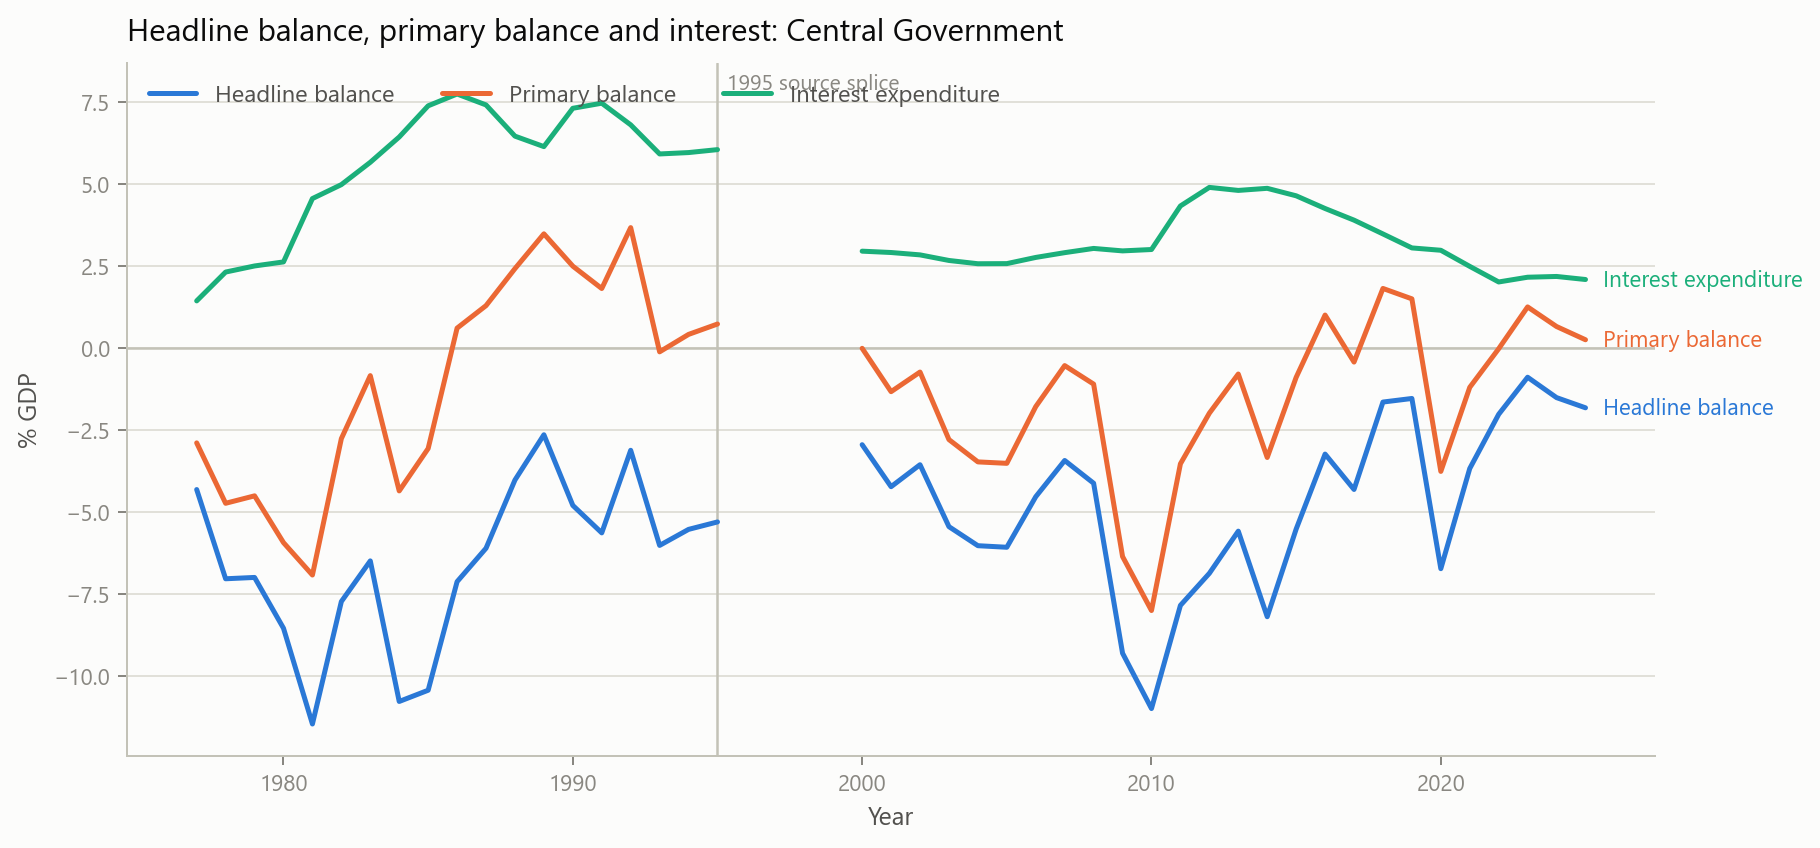
\includegraphics[width=\linewidth]{06_central_primary_balance.png}
\caption{Central Government headline and primary balances.}
\end{figure}

This decomposition isolates the accounting contribution of interest from the remainder of the balance. It is used only to separate interest expenditure from the remaining accounting balance.

\section{Fixed-Capital Formation Diagnostic}

The repository reports an explicitly non-official diagnostic

\[
B^{before\ GFCF}_{i,t} = B_{i,t} + GFCF_{i,t}.
\]

For Central Government in 2025, GFCF was \textbf{4828 M EUR}, and the analytical balance before GFCF was \textbf{-808 M EUR}. This does not redefine the official fiscal balance; it only quantifies the scale of fixed-capital formation relative to B.9.

\section{Debt and Stock-Flow Adjustment}

Debt dynamics need not equal minus the annual B.9 balance. The modern CFP tables allow the reconciliation

\[
\Delta Debt_t = -B_t + SFA_t,
\]

where \(SFA\) is the stock-flow adjustment. In 2025, General Government Maastricht debt was \textbf{89.67\% of GDP}, and the stock-flow adjustment was \textbf{2.03\% of GDP}.

\begin{figure}[htbp]
\centering
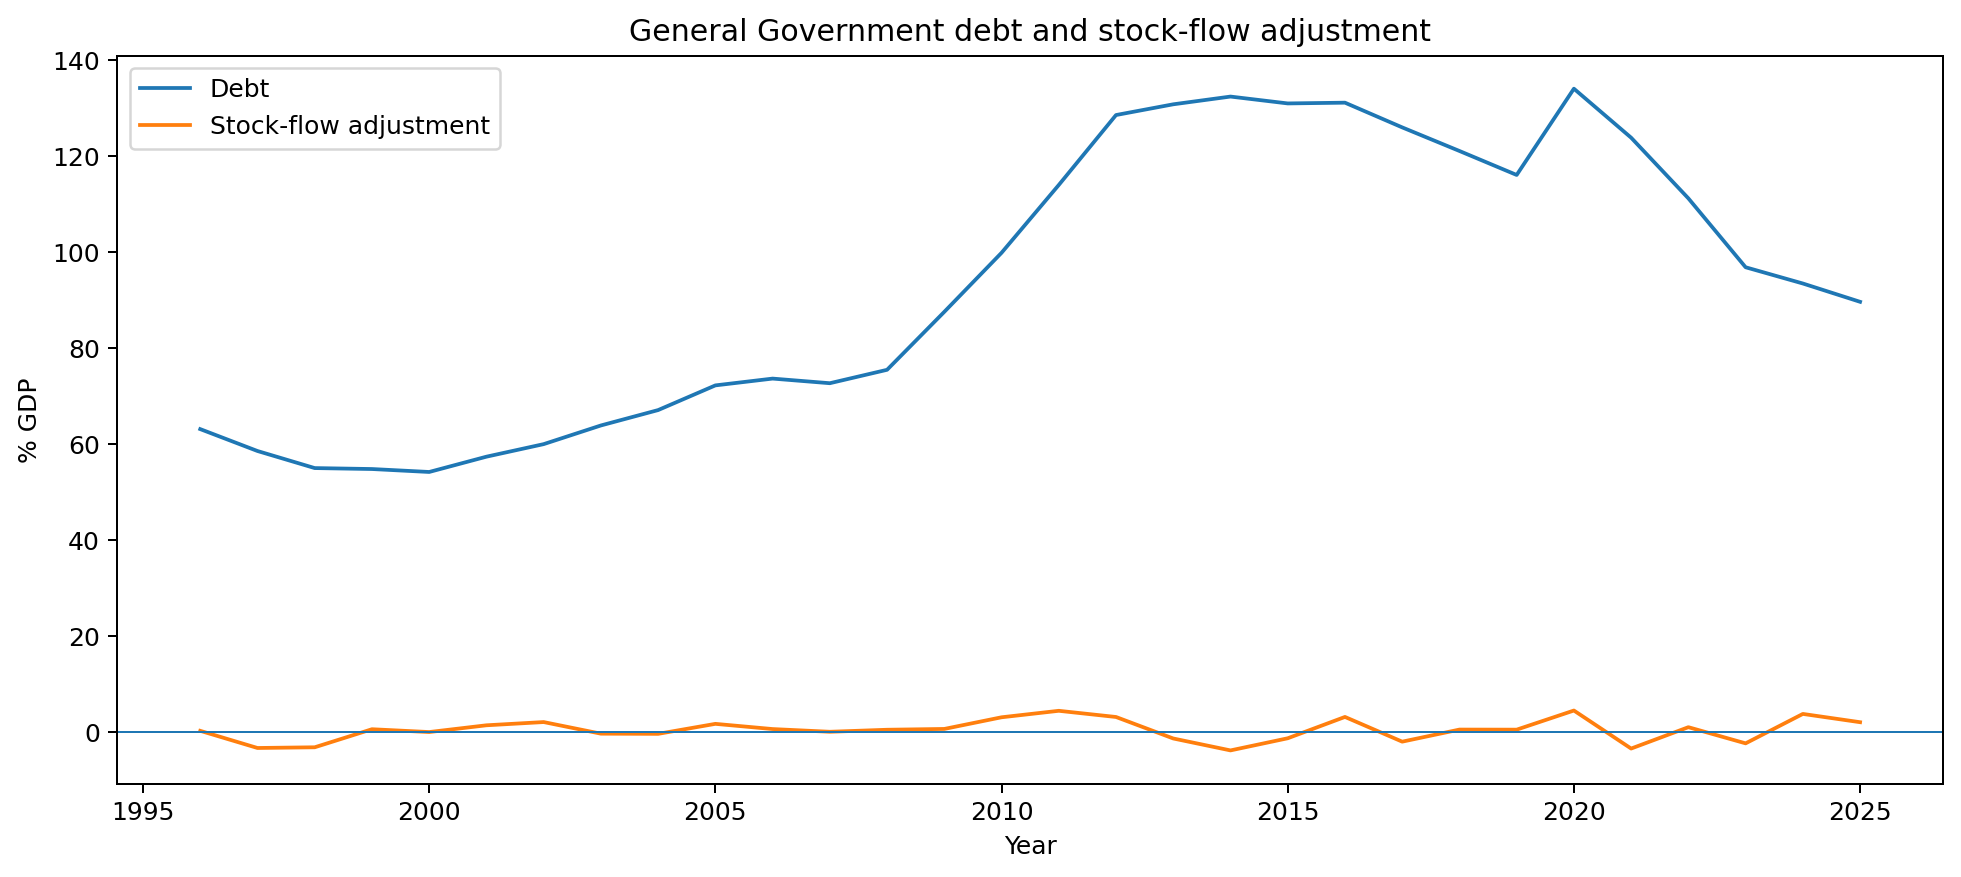
\includegraphics[width=\linewidth]{07_general_government_debt.png}
\caption{General Government debt and stock-flow adjustment.}
\end{figure}

\section{Persistence and Structural Mean Shifts}

Structural mean-shift detection is performed separately inside the 1977--1994 historical regime and the 1995--2025 modern regime. This prevents the known 1995 statistical splice from being mistaken for an economic break. A conservative piecewise-constant model with at most two breaks and a minimum five-year segment is selected by BIC.

\begin{center}
\resizebox{\linewidth}{!}{%
\begin{tabular}{@{}lllll@{}}
\toprule
regime & sector & n\_breaks & break\_years & segment\_means\_pct\_gdp \\
\midrule
1977-1994\_historical & general\_government & 1 & 1986 & -8.0942;-4.7630 \\
1977-1994\_historical & central\_government & 1 & 1987 & -8.1056;-4.7492 \\
1977-1994\_historical & regional\_local\_government & 0 &  & -0.2750 \\
1977-1994\_historical & social\_security\_funds & 0 &  & 0.4602 \\
1995-2025\_modern & general\_government & 2 & 2009;2015 & -4.3662;-7.9664;-1.4712 \\
1995-2025\_modern & central\_government & 2 & 2009;2016 & -4.4779;-7.7736;-2.7526 \\
1995-2025\_modern & regional\_local\_government & 2 & 2000;2011 & -0.0006;-0.4598;0.1550 \\
1995-2025\_modern & social\_security\_funds & 2 & 2016;2021 & 0.3522;1.0925;1.8804 \\
\bottomrule
\end{tabular}%
}
\end{center}

The detected dates are descriptive model outputs. The repository does not assign historical causes to them automatically.

\section{Descriptive Macroeconomic Co-Movement}

The full-period macroeconomic regression uses \textbf{nominal GDP growth}, because that variable can be reconstructed consistently from the bundled sources across 1977--2025. It is deliberately not described as an output gap or as a structural cyclical adjustment. HAC standard errors are used.

\begin{center}
\resizebox{\linewidth}{!}{%
\begin{tabular}{@{}lllllll@{}}
\toprule
sector & n & r\_squared & nominal\_gdp\_growth\_coef & nominal\_gdp\_growth\_se\_hac & nominal\_gdp\_growth\_pvalue\_hac & modern\_regime\_coef \\
\midrule
general\_government & 48 & 0.1751 & 7.7012 & 8.8215 & 0.3827 & 3.6653 \\
central\_government & 48 & 0.1634 & 5.5312 & 7.6465 & 0.4695 & 2.8982 \\
regional\_local\_government & 48 & 0.0807 & -0.0090 & 0.8348 & 0.9914 & 0.2213 \\
social\_security\_funds & 48 & 0.0707 & 2.1789 & 2.0029 & 0.2766 & 0.5458 \\
\bottomrule
\end{tabular}%
}
\end{center}

For 1978--1995 only, the historical Banco de Portugal / INE workbook also permits a small SSF model using employment growth and the unemployment rate:

\begin{center}
\resizebox{\linewidth}{!}{%
\begin{tabular}{@{}llllllll@{}}
\toprule
n & r\_squared & employment\_growth\_coef & employment\_growth\_se\_hac & employment\_growth\_pvalue\_hac & unemployment\_rate\_coef & unemployment\_rate\_se\_hac & unemployment\_rate\_pvalue\_hac \\
\midrule
18 & 0.2494 & 9.7252 & 5.2069 & 0.0618 & 20.2847 & 8.5997 & 0.0183 \\
\bottomrule
\end{tabular}%
}
\end{center}

These regressions quantify co-movement. They are not causal estimates.

\section{Intergovernmental Transfers}

Historical source tables identify current and capital transfers received and paid between public administrations. The repository computes a mechanical transfer-reallocation sensitivity:

\[
B^{sens}_{i,t}
=
B_{i,t}-(T^{received}_{i,t}-T^{paid}_{i,t}).
\]

This is intentionally not labelled an underlying or true balance. Removing a transfer while leaving the associated expenditure responsibility unchanged would generally not define a meaningful counterfactual.

\section{Methodological Limitations}

\begin{enumerate}
\item \textbf{1995 is a known source/methodology splice.} Both historical and modern 1995 values are retained in \path{data/interim/methodology_overlap_1995.csv}.
\item \textbf{Detailed subsector accounts have a 1996--1999 gap.} No interpolation is performed.
\item \textbf{Nominal GDP growth is not an output gap.} The full-period co-movement analysis should not be read as a cyclically adjusted balance.
\item \textbf{Social Security national accounts and budget-system accounts have different boundaries.} They are never merged into one balance series.
\item \textbf{The fixed-investment diagnostic is not an official balance concept.}
\item \textbf{Structural-break dates are statistical summaries, not causal event labels.}
\item \textbf{All interpretation is restricted to accounting, statistical and economic relationships directly supported by the data.}
\end{enumerate}

\section{Reproducibility}

The repository preserves raw source workbooks, source-specific intermediate CSVs, canonical processed datasets, analysis tables, figures, executed notebooks and SHA-256 hashes of every bundled raw file. The default execution is:

\begin{verbatim}
poetry install
make all
\end{verbatim}

The final report is regenerated from persisted analysis outputs rather than from hard-coded conclusions.

\end{document}
